\documentclass[a4paper,12pt]{article}
\usepackage[utf8]{inputenc}
\usepackage[spanish]{babel}
\usepackage{color}
\usepackage{parskip}
\usepackage{graphicx}
\usepackage{multirow}
\usepackage{listings}
\definecolor{mygreen}{rgb}{0,0.6,0}
\definecolor{lbcolor}{rgb}{0.9,0.9,0.9}

\lstset{
backgroundcolor=\color{lbcolor},
    tabsize=4,    
%   rulecolor=,
    language=[GNU]C++,
        basicstyle=\scriptsize,
        aboveskip={1.5\baselineskip},
        columns=fixed,
        showstringspaces=false,
        extendedchars=false,
        breaklines=true,
        prebreak = \raisebox{0ex}[0ex][0ex]{\ensuremath{\hookleftarrow}},
        frame=single,
        showtabs=false,
        showspaces=false,
        showstringspaces=false,
        identifierstyle=\ttfamily,
        keywordstyle=\color[rgb]{0,0,1},
        commentstyle=\color[rgb]{0.026,0.112,0.095},
        stringstyle=\color{red},
        numberstyle=\color[rgb]{0.205, 0.142, 0.73},
%        \lstdefinestyle{C++}{language=C++,style=numbers}’.
}


\begin{document}



\section{Problema}

Hacer una calculadora que procese operaciones simples utilizando la estructura de datos Pila.

\section{Código}

\subsection{Pila.h}

\begin{lstlisting}
#ifndef PILA_H
#define PILA_H

template<typename T>
class Pila
{
    public:
        Pila();
        class Nodo{
            public:
                Nodo();
                Nodo(T dato);prosece
                T dato;
                Nodo *siguiente;
            private:
        };
        void agregar(T dato);
        bool esVacia();
        T desapilar();
    protected:
    private:
        Nodo * cabeza;
};

template<typename T>
Pila<T>::Nodo::Nodo(){
    siguiente = nullptr;
}
template<typename T>
Pila<T>::Nodo::Nodo(T dato){
    this->dato = dato;
}
template<typename T>
Pila<T>::Pila(){
    cabeza = nullptr;
}
template<typename T>
void Pila<T>::agregar(T dato){
    Pila<T>::Nodo * nuevo = new Nodo(dato);
    if(cabeza == nullptr){
        cabeza = nuevo;
    }
    else{
        nuevo->siguiente = cabeza;
        cabeza = nuevo;
    }
}
template<typename T>
bool Pila<T>::esVacia(){
    if(cabeza == nullptr)
        return true;
    return false;
}
template<typename T>
T Pila<T>::desapilar(){
    if(esVacia()){
        return 0;
    }
    else{
        T result = cabeza->dato;
        cabeza = cabeza->siguiente;
        return result;
    }
}

#endif // PILA_H

\end{lstlisting}

\subsection{main.cpp}

\begin{lstlisting}

#include <iostream>
#include <Pila.h>
#include <math.h>

using namespace std;

float convertirNumero(string numero){
    double resultado = 0;
    auto iter = numero.end();
    iter--;
    double contador = 0;
    for(iter; iter!= numero.begin(); iter--){
        if((*iter) == '.'){
            resultado /= pow(10,contador);
            contador = -1;
        }
        else{
            resultado += pow(10,contador) * ((*iter) - 48);
        }
        contador++;
    }
    resultado += pow(10,contador) * ((*iter) - 48);
    return resultado;
}
int main()
{
    Pila<float> memoria;
    string expresion;
    string temp;
    cin>>expresion;
    for(int i = 0; i < expresion.size(); i++){
        if(expresion[i] == '|'){
            memoria.agregar(convertirNumero(temp));
            temp.clear();
        }
        else if((expresion[i] >= 48 and expresion[i] <= 57)
                 or expresion[i] == '.'){
            temp.insert(temp.end(),expresion[i]);
        }
        else{
            switch(expresion[i]){
                case '+':
                    memoria.agregar(memoria.desapilar()
                                     + convertirNumero(temp));
                    temp.clear();
                    break;
                case '-':
                    memoria.agregar(memoria.desapilar()
                                     - convertirNumero(temp));
                    temp.clear();
                    break;
                case '*':
                    memoria.agregar(memoria.desapilar()
                                     * convertirNumero(temp));
                    temp.clear();
                    break;
                case '/':
                    memoria.agregar(memoria.desapilar()
                                     / convertirNumero(temp));
                    temp.clear();
                    break;
                default:
                    cout<<"El caracter "<<expresion[i]
                        <<" no se puede reconocer";
                    return 0;
            }
        }
    }
    cout<<memoria.desapilar();
}

\end{lstlisting}

\onecolumn

\section{Ejemplo}

\begin{figure}[h]
 \centering
 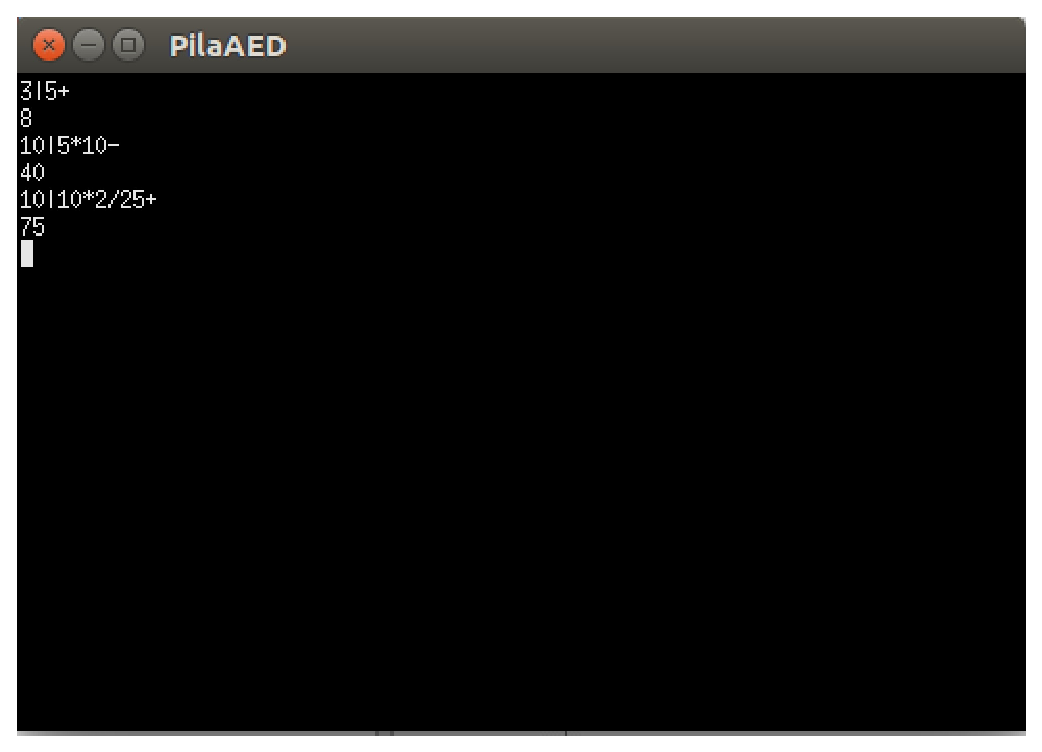
\includegraphics[scale=0.5]{imagenes/1.eps}
 \caption{EJemplo}
\end{figure}


\end{document}


